\documentclass[pdflatex,sn-mathphys-num]{sn-jnl}% Math and Physical Sciences Numbered Reference Style
% Source-review markers are no-op by default and are not printed.
\providecommand{\reviewermap}[3]{}
%%\documentclass[pdflatex,sn-mathphys-ay]{sn-jnl}% Math and Physical Sciences Author Year Reference Style
%%\documentclass[pdflatex,sn-aps]{sn-jnl}% American Physical Society (APS) Reference Style
%%\documentclass[pdflatex,sn-vancouver-num]{sn-jnl}% Vancouver Numbered Reference Style
%%\documentclass[pdflatex,sn-vancouver-ay]{sn-jnl}% Vancouver Author Year Reference Style
%%\documentclass[pdflatex,sn-apa]{sn-jnl}% APA Reference Style
%%\documentclass[pdflatex,sn-chicago]{sn-jnl}% Chicago-based Humanities Reference Style

%%%% Standard Packages
%%<additional latex packages if required can be included here>

\usepackage{graphicx}%
\usepackage{multirow}%
\usepackage{amsmath,amssymb,amsfonts}%
\usepackage{amsthm}%
\usepackage{mathrsfs}%
\usepackage[title]{appendix}%
\usepackage{xcolor}%
\usepackage{textcomp}%
\usepackage{manyfoot}%
\usepackage{booktabs}%
\usepackage{algorithm}%
\usepackage{algorithmicx}%
\usepackage{algpseudocode}%
\usepackage{listings}%

% User defined
%%%%Userd-added package
\usepackage[version=3]{mhchem}
\usepackage{subcaption}
\usepackage{graphicx}
\usepackage{float}
\usepackage{multirow}
\usepackage{array}
\usepackage{amsmath}
\usepackage{booktabs}
\usepackage{amsmath}
\usepackage{amssymb}
\usepackage{xcolor}

\usepackage[utf8]{inputenc} % allow utf-8 input
\usepackage{hyperref}       % hyperlinks
\usepackage{url}            % simple URL typesetting
\usepackage{amsfonts}       % blackboard math symbols
\usepackage{nicefrac}       % compact symbols for 1/2, etc.
\usepackage{microtype}      % microtypography
\usepackage{lineno}

%%%%
%% as per the requirement new theorem styles can be included as shown below
\theoremstyle{thmstyleone}%
\newtheorem{theorem}{Theorem}%  meant for continuous numbers
%%\newtheorem{theorem}{Theorem}[section]% meant for sectionwise numbers
%% optional argument [theorem] produces theorem numbering sequence instead of independent numbers for Proposition
\newtheorem{proposition}[theorem]{Proposition}% 
%%\newtheorem{proposition}{Proposition}% to get separate numbers for theorem and proposition etc.

\theoremstyle{thmstyletwo}%
\newtheorem{example}{Example}%
\newtheorem{remark}{Remark}%

\theoremstyle{thmstylethree}%
\newtheorem{definition}{Definition}%

% Supplementary numbering
\setcounter{figure}{0}
\renewcommand{\thefigure}{S\arabic{figure}}
\setcounter{table}{0}
\renewcommand{\thetable}{S\arabic{table}}
\raggedbottom
%%\unnumbered% uncomment this for unnumbered level heads

\begin{document}
\linenumbers

\title[Article Title]{Supplementary Information: Non-Equilibrium Probes Reveal the Limits of Specialist and Foundation Machine-Learned Force Fields}

%%=============================================================%%
%% GivenName	-> \fnm{Joergen W.}
%% Particle	-> \spfx{van der} -> surname prefix
%% FamilyName	-> \sur{Ploeg}
%% Suffix	-> \sfx{IV}
%% \author*[1,2]{\fnm{Joergen W.} \spfx{van der} \sur{Ploeg} 
%%  \sfx{IV}}\email{iauthor@gmail.com}
%%=============================================================%%

\author[1]{\fnm{Yi} \sur{Cao}}\email{ycao73@jh.edu}

\author[1]{\fnm{Peter} \sur{Mastracco}}\email{pmastra2@jh.edu}
% \author[1]{\fnm{Victor} \sur{Wu}}\email{vwu16@jhu.edu}
% % \equalcont{These authors contributed equally to this work.}

\author*[1]{\fnm{Paulette} \sur{Clancy}}\email{pclancy3@jhu.edu}
% \equalcont{These authors contributed equally to this work.}

\affil*[1]{\orgdiv{Department of Chemical and Biomolecular Engineering}, \orgname{ Johns Hopkins University}, \orgaddress{\street{3400 N. Charles Street}, \city{Baltimore}, \postcode{21218}, \state{Maryland}, \country{USA}}}


%%\pacs[JEL Classification]{D8, H51}

%%\pacs[MSC Classification]{35A01, 65L10, 65L12, 65L20, 65L70}

\maketitle

\section*{Supplementary Information Roadmap}
\reviewermap{REV-A1/REV-A2/REV-A6/REV-C8/REV-C9/REV-C10/REV-C11/REV-C12/REV-C13}{done-local}{SI roadmap added to connect reference calculations, data provenance, task probes, and interpretability checks.}
This Supplementary Information is organized to make the benchmark traceable from reference calculations to model evaluation. Section~1 describes the first-principles setup, NEB reference protocol, MACE training configurations, dataset provenance, and split controls. Section~2 provides the supporting analyses: RMSE benchmarking, structural and thermodynamic validation, molecular-dynamics property calculations, representation-learning descriptors, migration-path diagnostics, self-consistent MLFF-NEB tests, and SHAP surrogate interpretation. Together, these sections separate three observables that are otherwise easy to conflate: the DFT reference barrier on a converged path, the MLFF energy assigned to a fixed DFT path, and the barrier obtained after a model relaxes its own path.

\paragraph{Audit trail.}
\reviewermap{REV-C8/REV-C13}{done-local}{Added explicit source-ledger hook for numerical claims, figures, and tables.}
Numerical values and revised figures are tracked in the source ledger \texttt{Revision1/data\_processed/manuscript\_source\_ledger.csv}. The ledger records the manuscript location, displayed value, source table or script, and current evidence status. It is checked by \texttt{Revision1/scripts/audit\_manuscript\_sources.py}, which verifies that referenced figures/tables exist and that ledgered claim tokens are present in the current \texttt{Revision1} manuscript sources.


\newcommand{\pc}[1]{{\color{purple}[Paulette: #1]}}
\newcommand{\yi}[1]{{\color{orange!80}[Yi: #1]}}


\section{Detailed Computational Methods}
\subsection{First-Principles Reference Calculations}
% All DFT calculations were performed using the \textsc{Quantum ESPRESSO} package~\cite{giannozzi2009quantum}. The exchange-correlation interaction was treated using the Perdew–Burke–Ernzerhof (PBE) functional within the generalized gradient approximation (GGA)~\cite{perdew1996generalized}. To accurately capture the long-range van der Waals (vdW) interactions that are critical to represent in layered materials, dispersion corrections were included \textit{via} the Grimme DFT-D3 scheme.  
% We employed ultrasoft pseudopotentials for all elements (Cr, Sb, Te) with a plane-wave kinetic energy cutoff of 400 eV. The Brillouin zone was sampled using a Monkhorst-Pack k-point grid of $4 \times 4 \times 1$ for structural relaxations and Nudged Elastic Band (NEB) calculations. 

All first-principles calculations were performed using the \textsc{Quantum ESPRESSO} package~\cite{giannozzi2009quantum}. The exchange–correlation energy was described using the Perdew–Burke–Ernzerhof (PBE) functional within the generalized gradient approximation (GGA)~\cite{perdew1996generalized}. Long-range dispersion interactions, essential for accurately representing the interlayer physics of \ce{Sb2Te3}, were included through the Grimme DFT-D3 correction scheme. Spin–orbit coupling (SOC) was incorporated through fully relativistic ONCV pseudopotentials (SG15 v1.2).

A plane-wave kinetic energy cutoff of 100~Ry and a charge density cutoff of 400~Ry were used for all calculations. Electronic occupations were treated with the cold-smearing scheme using a smearing width of 0.0147~Ry, which provides stable convergence for narrow-gap chalcogenides. Electronic states were iterated until the total electronic energy converged below $10^{-6}$~Ry, using a mixing parameter of 0.4 and a maximum of 200 electronic iterations per self-consistent cycle.

All structural relaxations were performed using the Broyden–Fletcher–Goldfarb–Shanno (BFGS) algorithm for both ionic and cell degrees of freedom, with force and pressure convergence thresholds of $10^{-3}$~Ry/Bohr and 0.5~kbar, respectively. A uniform Monkhorst–Pack mesh of $4 \times 4 \times 1$ was employed to sample the Brillouin zone for relaxations and Nudged Elastic Band (NEB) calculations. The $4 \times 2 \times 1$ supercell with dopant contained 81 atoms, corresponding to a two-quintuple-layer (2QL) slab of \ce{Sb2Te3} with one interstitial Cr atom, separated by sufficient vacuum to avoid spurious periodic interaction. Restart files were written periodically to ensure computational stability during long relaxations.


\reviewermap{REV-A1}{partial}{DFT NEB references must include per-path convergence status; current path 1-4 reference candidate is 0.336050 eV.}
The training dataset was generated from ab initio molecular dynamics (AIMD) simulations performed in the NVT ensemble using a Langevin thermostat. These simulations covered a range of temperatures (300 K, 600 K, 1200 K) and Cr doping concentrations to ensure the model was exposed to a diverse set of thermodynamic and structural configurations. Each AIMD trajectory was run for 10 ps on a system of 120 atoms. To investigate the nature of atomic migration pathways, minimum energy paths (MEPs) and energy barriers were calculated using the Nudged Elastic Band (NEB) method. In the accompanying data release, each NEB path is reported with its task label, number of images, input structure provenance, restart lineage, convergence threshold, achieved maximum force, and activation barrier. Paths that are not yet formally converged are marked as candidate references and are excluded from final ranking until the corresponding restarted QE calculation reaches the stated criterion [PLACEHOLDER: final NEB convergence table].

% \subsection{MACE Model Training Protocols}
% \subsubsection{Training Hyperparameters}
% All training and fine-tuning procedures were executed with a consistent set of hyperparameters to ensure fair comparison:
% \begin{itemize}
%     \item Optimizer: Adam
%     \item Initial learning rate: $1\times10^{-3}$
%     \item Batch size: 32
%     \item Early stopping: Implemented based on validation set Force MAE
%     \item Maximum epochs: 1000
%     \item Validation split: 10\% of training data
% \end{itemize}

% \subsubsection{Fine-Tuning Details}
% For the FT-Multi\_T model, the training subset was composed equally from 300K, 600K, and 1200K trajectories, ensuring exposure to diverse thermal conditions. The multi-temperature dataset was designed to test whether broader thermodynamic sampling improves generalization.

% For the FT-600K model, we selected a representative 5\% subset (approximately 1,000 configurations) from the 600K AIMD trajectories. The subset was chosen to capture the full range of structural variations observed at this temperature, including both equilibrium fluctuations and transitional configurations. Model training and fine-tuning were focused at 600 K, as this temperature is representative of typical thermoelectric operating conditions. At roughly two-thirds of Sb$_2$Te$_3$'s melting point, this temperature captures significant thermal dynamics without structural deterioration.

% Fine-tuning foundation models for specific chemical systems presents a fundamental challenge: how to adapt to new domains while preserving learned representations. This document discusses our fine-tuning strategy.


\subsection{MACE Model Training Protocols}

\subsubsection{Training Hyperparameters}
All training and fine-tuning procedures were performed with consistent hyperparameters to ensure direct comparability. Unless otherwise stated, we used the Adam optimizer with an initial learning rate of $1\times10^{-3}$, a batch size of 32, a maximum of 1000 epochs, and early stopping based on validation-set force MAE. A 10\% validation split was applied to all datasets.

Fine-tuning was initialized from the \texttt{MACE-MP-0 (PBE)}~\cite{batatia_mace_nodate} foundation model. All model parameters were updated without freezing any layers, and all output heads were fine-tuned using the standard multi-head strategy. Stochastic Weight Averaging (SWA) was activated from epoch 100, and Exponential Moving Average (EMA) tracking ($\alpha=0.99$) was applied throughout training. Energy and forces were read using the keys \texttt{energy} and \texttt{forces}, respectively, with force, energy, and stress loss weights of 100.0, 1.0, and 0.0. The training configuration employed $l_{\max}=2$, cutoff radius $r_{\max}=6.0$~Å.
\reviewermap{REV-C8}{pending-local}{Final release will include the exact extraction script, input key mapping, and dataset checksum for each model-training file.}
Every training dataset is registered in the MigrationBench manifest with its source trajectory, frame-selection rule, split assignment, random seed, energy/force key mapping, and checksum [PLACEHOLDER: final dataset manifest DOI or Hugging Face commit hash]. This provenance layer makes the energy and force extraction path auditable from raw DFT output to model-training file.

% To stabilize multi-head finetuning, we incorporated 1000 FPS-selected structures from the pretraining dataset, weighted at 1.0 for the replay head. Identical optimizer settings, loss definitions, learning rate schedules, and train/validation/test splits were used for both FT-600K and FT-Multi\_T.

\subsubsection{Fine-Tuning Details}
The multi-temperature fine-tuning model (FT-Multi\_T) was constructed by combining configurations at 300~K, 600~K, and 1200~K. Each configuration was simulated at all three temperatures, ensuring that the Multi\_T dataset is strictly balanced across temperatures without statistical or configurational bias. This design probes whether broader thermodynamic sampling improves model robustness and generalization.

For the 600~K single-temperature fine-tuning model (FT-600K), we selected exactly 5\% of frames from the 600~K AIMD trajectories. Subsampling was performed independently for each trajectory via uniform temporal downsampling (i.e., retaining every $N$th step), which is equivalent to uniform random sampling due to the absence of periodic temporal correlations. The subsampled frames were merged into a single dataset containing approximately 1000 configurations. This subset captures the full structural variability at 600~K, a temperature representative of realistic thermoelectric operating conditions, lying near two-thirds of the melting point of Sb$_2$Te$_3$ and exhibiting significant anharmonic dynamics without structural degradation.

\reviewermap{REV-A2/REV-C10}{pending}{Grouped split and train/test overlap audit must be documented once SOAP/RMSD values are available.}
Both FT-600K and FT-Multi\_T models were compared using the same split-generation rule so that differences between models are not produced by repartitioning alone. Splits are assigned at the trajectory/configuration-family level rather than independently per frame, preventing near-duplicate structures from appearing in both training and test partitions. We additionally audit benchmark-path proximity using nearest-neighbor SOAP distance and Cartesian RMSD to the training set [PLACEHOLDER: FT-600K and FT-Multi-T nearest-neighbor SOAP/RMSD statistics]. These values will be reported with the final benchmark-path proximity table.
% corresponding structures occupy identical partitions in both cases.

% Fine-tuning foundation models for chemically complex chalcogenides requires balancing adaptation to new bonding motifs against preservation of transferable learned representations. The unified protocol described above provides a controlled and reproducible framework for evaluating domain adaptation across temperatures and data regimes.


% \subsubsection{Fine-tuning Underlying Mechanism}

% In fine-tuning, the pre-trained model parameters $\theta_0$ are directly optimized on the target dataset $\mathcal{D}_{\text{target}}$:

% \begin{equation}
% \theta^* = \arg\min_\theta \mathcal{L}(\theta; \mathcal{D}_{\text{target}})
% \end{equation}




% \paragraph{Characteristics}
% \begin{itemize}
%     \item \textbf{Simple implementation}: Direct optimization on new data
%     \item \textbf{Fast convergence}: High learning rate ($\alpha \sim 10^{-2}$)
%     \item \textbf{Catastrophic forgetting}: Loss of original capabilities
%     \item \textbf{Single objective}: Optimizes only for target domain performance
% \end{itemize}

% \subsubsection{Implementation Details}

% \subsubsection{Fine-tuning Algorithm}

% \begin{algorithm}
% \caption{Fine-tuning}
% \begin{algorithmic}
% \STATE Initialize: $\theta \leftarrow \theta_{\text{foundation}}$
% \FOR{epoch = 1 to $N_{\text{epochs}}$}
%     \FOR{batch $\in \mathcal{D}_{\text{target}}$}
%         \STATE $\mathcal{L} \leftarrow \text{MSE}(f_\theta(\text{batch}), y_{\text{batch}})$
%         \STATE $\theta \leftarrow \theta - \alpha \nabla_\theta \mathcal{L}$
%     \ENDFOR
% \ENDFOR
% \end{algorithmic}
% \end{algorithm}

% \subsubsection{Practical Considerations}

% \paragraph{When to Use Fine-tuning}
% \begin{itemize}
%     \item Limited computational resources
%     \item Domain-specific applications only
%     \item Rapid prototyping requirements
%     \item No need for generalization beyond the target dataset
% \end{itemize}

% \paragraph{Take-away}

% Fine-tuning offers rapid adaptation to new datasets with relatively low computational cost. However, naive fine-tuning comes at the expense of catastrophic forgetting, where the model loses its original generalization capabilities.



\section{Supplementary Materials}
\subsection{MACE Model Performance Evaluation by RMSE}

All developed Machine-Learned Force Fields (MLFFs) demonstrate high fidelity in predicting energies and forces, as illustrated by the parity plots in Figure~\ref{fig:mace_parity}, which compare model predictions to the reference DFT calculations. The performance of each model across the training, validation, and test sets is quantitatively summarized in Table~\ref{tab:mace_performance_detailed}. As detailed in the table, the models fine-tuned from the foundation model show a marked improvement over the model trained from scratch, with energy and force Root Mean Square Errors (RMSEs) being significantly reduced on the independent test set.

\begin{table}[htbp]
    \centering
    \caption{Performance metrics for MACE models across training, validation, and test sets. The FT-600K metrics are the mean $\pm$ standard deviation across three independent training runs with different random seeds.}
    \label{tab:mace_performance_detailed}
    \begin{tabular}{lcccc}
        \toprule
        \textbf{Model} & \textbf{Train RMSE F} & \textbf{Valid RMSE F} & \textbf{Test RMSE F} & \textbf{Test RMSE E} \\
         & (meV/\AA) & (meV/\AA) & (meV/\AA) & (meV/atom) \\
        \midrule
        From Scratch & 67.1 & 76.1 & 75.2 & 1.0 \\
        FT-600K & 20.7 $\pm$ 11.8 & 44.6 $\pm$ 2.9 & 37.2 $\pm$ 0.6 & 0.5 $\pm$ 0.0 \\
        FT-MultiT & 20.3 & 49.1 & 45.5 & 0.5 \\
        \bottomrule
    \end{tabular}
\end{table}

A deeper analysis of the training dynamics reveals important characteristics of the models. The model trained from scratch exhibits a relatively small gap between training (67.1 meV/\AA) and validation (76.1 meV/\AA) force RMSEs. While this suggests only moderate overfitting, its high error across all datasets indicates that it underfits the true physical interactions.

In contrast, the fine-tuned models display a more pronounced overfitting behavior, characterized by a large gap between their low training RMSEs and higher validation RMSEs. For instance, the FT-MultiT model shows a 142\% increase in force RMSE from the training (20.3 meV/\AA) to the validation set (49.1 meV/\AA). This aggressive fitting is expected when fine-tuning on smaller, more specialized datasets. The high standard deviation in the FT-600K model's training RMSE (11.8 meV/\AA) also suggests a sensitivity to initialization during the training process.

Despite the strong overfitting signals, the fine-tuned models generalize well to the test set, outperforming the scratch model by a significant margin. This analysis reinforces the central argument of our work: standard accuracy metrics like RMSE are insufficient for a comprehensive evaluation of MLFFs. While these metrics and the parity plots in Figure~\ref{fig:mace_parity} confirm the models' general accuracy, they do not capture critical performance on physical properties such as energy barriers and transport phenomena, necessitating the more extensive, property-driven benchmarks presented in the main text.

\begin{figure}[ht]
    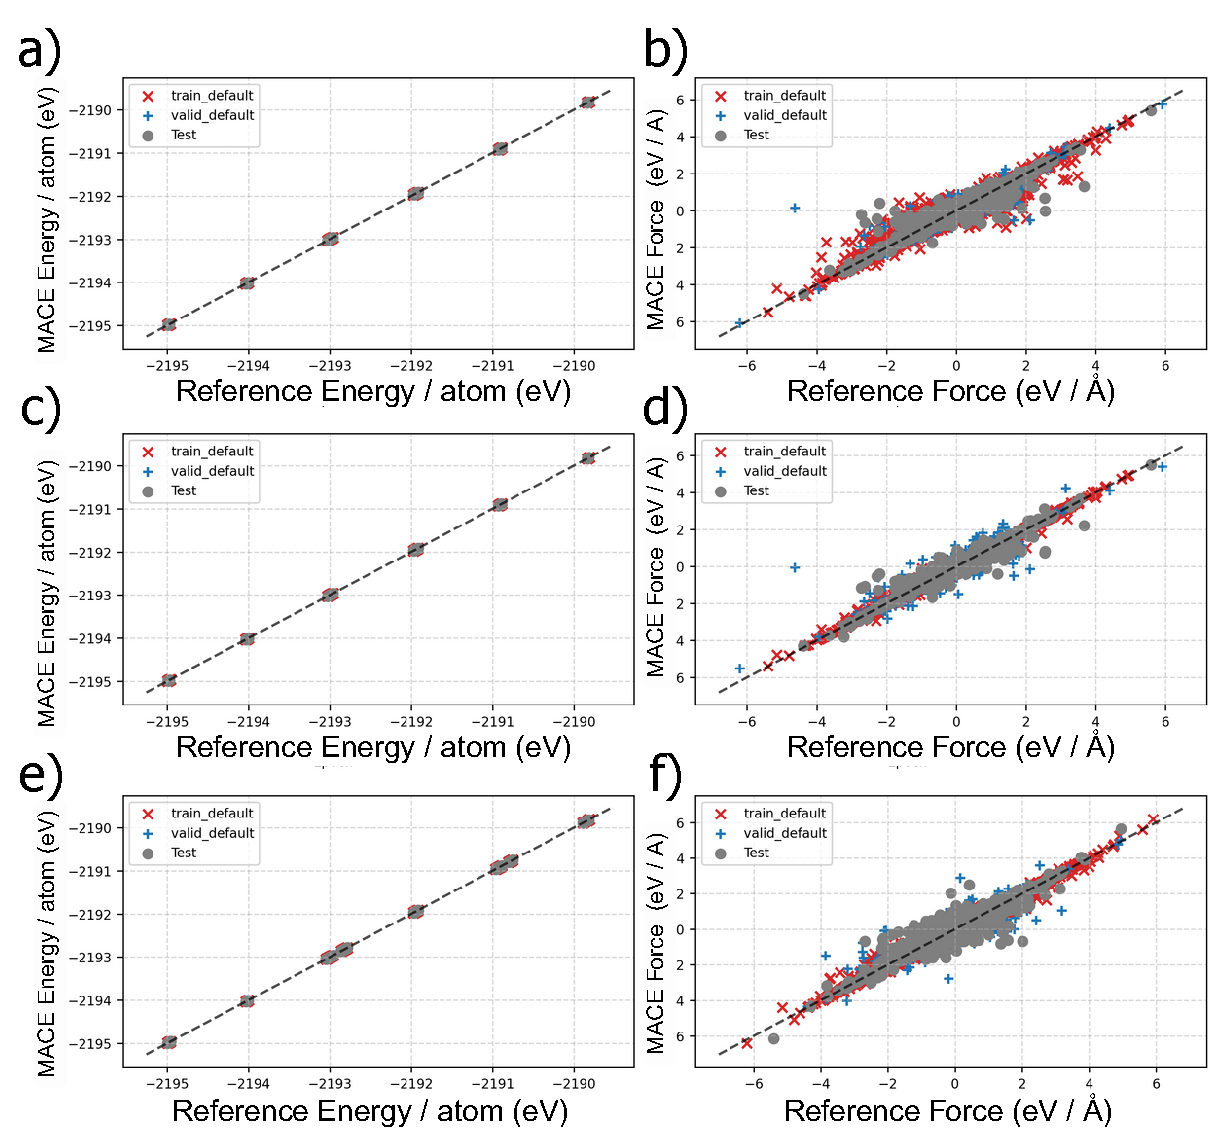
\includegraphics[width=0.8\textwidth]{Fig/NeurIPS2025-AI4MAT-SI1.pdf}
    \centering
    \caption{\textbf{Parity plots comparing MACE-predicted energies and forces against DFT reference calculations for the test set.} (a, b) Model trained from scratch, (c, d) fine-tuned 600 K model (``FT-600K''), and (e, f) fine-tuned multi-temperature model (``FT-MultiT''). Parity plots for energies (a, c, e) demonstrate excellent agreement for all models, while force parity plots (b, d, f) show strong overall correlation but subtle differences in error distributions that are not distinguishable visually. These results highlight the necessity of quantitative and property-based benchmarks for robust model evaluation.}
    \label{fig:mace_parity}
\end{figure}





\subsection{Detailed Structural and Thermodynamic Analysis}
The RDF analysis reveals that all MACE models, regardless of training strategy, successfully reproduce the key structural features of the Cr-doped Sb$_2$Te$_3$ system when compared to the AIMD ground truth (Fig.~\ref{fig:rdf}b).

All models correctly capture the primary coordination shells, with the first peak positions for Cr--Cr, Cr--Sb, and Cr--Te pairs occurring at approximately 3.0~\AA, 3.2~\AA, and 2.8~\AA, respectively, in excellent agreement with the AIMD reference. The peak heights and positions remain consistent across all training strategies (Figures~\ref{fig:rdf}c--f), indicating that the local atomic structure is well preserved regardless of whether the model was trained from scratch, used as a foundation model, or fine-tuned with temperature-specific data.

The primary observable difference between models lies in the smoothness of the RDF curves rather than their fundamental features. The scratch-trained model (Fig.~\ref{fig:rdf}d) exhibits slightly smoother RDF profiles compared to the fine-tuned variants (Figures~\ref{fig:rdf}e--f). This difference arises from practical computational considerations rather than fundamental accuracy: the scratch model, being more compact with fewer parameters, allowed for longer MD trajectories within the same computational budget, resulting in better statistical sampling. In contrast, the fine-tuned models, while maintaining larger parameter counts from their foundation architectures, required more computational resources per MD step, limiting the total simulation time and resulting in slightly noisier RDF profiles.

% Notably, both fine-tuning strategies---whether using single-temperature (600~K) or multi-temperature AIMD data---produce nearly identical RDF profiles, suggesting that the structural representation of the material is robust to the temperature range of the training data. This indicates that, for structural properties, the choice of training strategy has minimal impact, with all approaches converging to similar descriptions of the local atomic environment. The preservation of accurate structural features across all models provides confidence that the learned interatomic potentials correctly capture the fundamental bonding characteristics of the Cr-doped Sb$_2$Te$_3$ system.

Notably, both fine-tuning strategies—whether using single-temperature (600 K) or multi-temperature AIMD data—yield RDF profiles that are nearly indistinguishable for this Cr-doped Sb$_2$Te$_3$ system. Within the scope of this test case, this similarity suggests that the structural descriptors learned by the models are not strongly sensitive to the temperature range of the fine-tuning dataset. While this observation is system-specific, it indicates that, for the structural properties examined here, the different training strategies converge to comparable representations of the local atomic environment. The consistent reproduction of key RDF features across all models supports the conclusion that each MLFF captures the essential bonding motifs relevant to this particular material.



\begin{figure}[ht]
    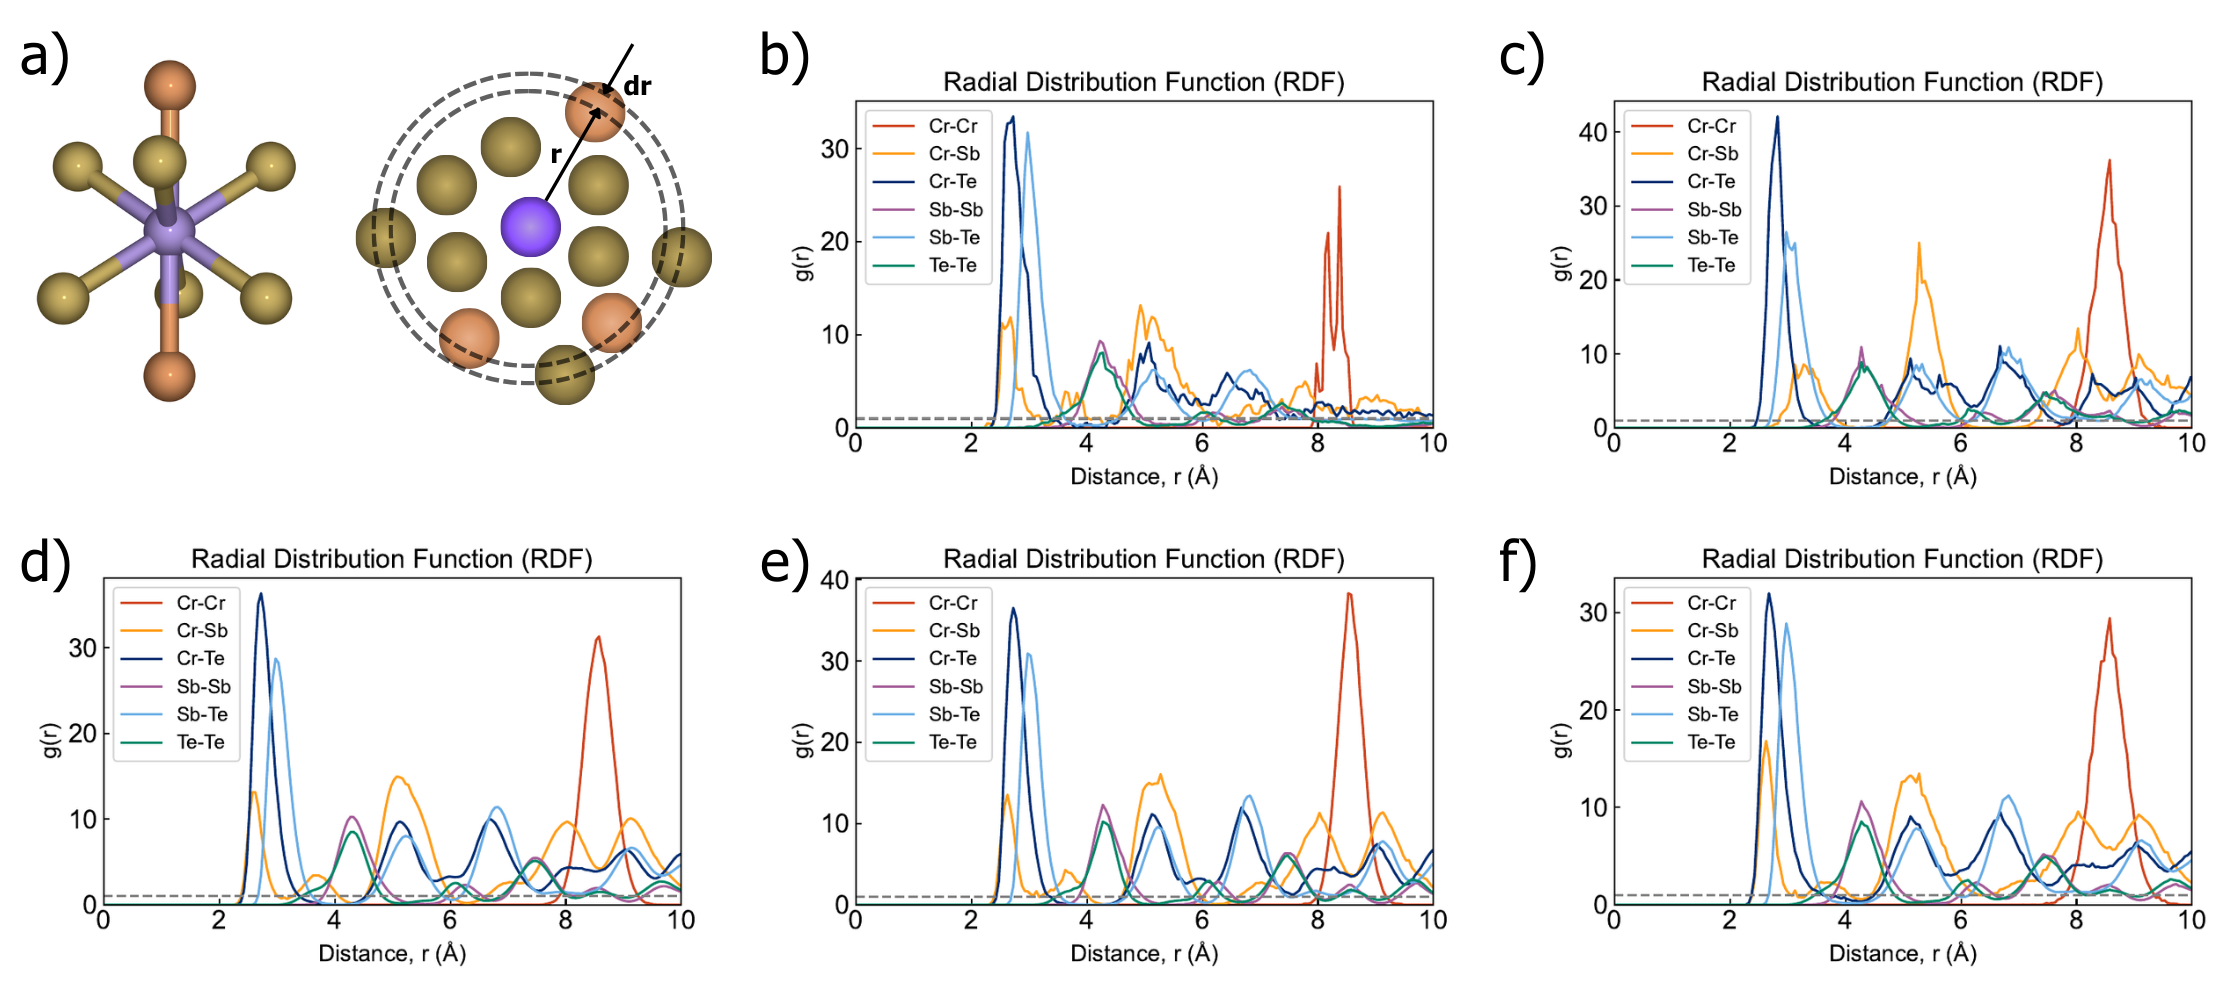
\includegraphics[width=0.8\textwidth]{Fig/NeurIPS2025-AI4MAT-figure2.png}
    \centering
    \caption{\textbf{Radial distribution function (RDF) analysis of Cr-doped Sb$_2$Te$_3$ at 600 K.} (a) Schematic illustration of the local atomic environment around a Cr dopant (purple) in the Sb$_2$Te$_3$ lattice, showing the first coordination shell of Te atoms (gold) and second-shell Sb atoms (orange). The dashed circles indicate the radial distances used for RDF calculation. (b-f) Computed RDFs for different atom pairs from molecular dynamics simulations: (b) Ab initio molecular dynamics (AIMD) ground truth reference, (c) MACE foundation model without fine-tuning, (d) MACE model trained from scratch on Cr-Sb$_2$Te$_3$ data, (e) MACE model fine-tuned with 600 K AIMD data (``FT - 600K''), and (f) MACE model fine-tuned with multi-temperature AIMD data (``FT - Multi-T''). All simulations were performed at 600 K with 5$\times$5$\times$1 supercells for 200 ps. The RDF peaks correspond to characteristic interatomic distances in the doped structure, with the first peak representing nearest-neighbor correlations.}
    \label{fig:rdf}
\end{figure}

\subsection{Thermodynamic Ensemble Stability}
A detailed analysis of the pressure profiles reveals subtle but important differences between models. The zero-shot MACE Foundation model equilibrates to a slightly different average pressure than the models trained or fine-tuned on our in-house AIMD data. This is likely a consequence of the foundation model being trained on a vast dataset of materials at their 0K equilibrium volumes. A minor mismatch between the foundation model's predicted equilibrium lattice parameters and the true DFT values for our specific Cr:Sb$_2$Te$_3$ system at 600K manifests as a persistent non-zero average pressure in an NVT simulation. The fine-tuned and scratch models, having been trained explicitly on data from this system's true ensemble, do not exhibit this deviation.

\subsection{Transport Property Analysis}
The divergence in transport properties provides deeper insights into model behavior. The enhanced diffusivity in multi-temperature fine-tuned models likely stems from their exposure to high-temperature configurations approaching disordered or liquid-like states during training. By learning from these states, the model may have developed a potential energy surface that is slightly "flatter" or has lower barriers to diffusion, an effect that persists even at the 600K simulation temperature.

The thermal conductivity analysis reveals even more fundamental differences. The rapid decay of thermal conductivity in the foundation model indicates a failure to sustain long-range heat-carrying vibrational modes (phonons) specific to this crystalline structure. The anomalous peak observed in the 600K-only fine-tuned model's HFACF during the first 50 ps suggests potential structural instability or abrupt structural changes that alter phonon behavior. This highlights how different training strategies can lead to qualitatively different representations of collective phenomena, even when local properties appear identical.

\begin{table}[htbp]
    \centering
    \caption{\textbf{Audited molecular-dynamics transport metrics.} Values are computed from the Revision~1 local re-analysis with block uncertainties. The FT-600K transport trajectory remains quarantined because the current local source corresponds to the shorter naive-FT run rather than the corrected long-run protocol.}
    \label{tab:md_transport_revised}
    \begin{tabular}{lllll}
\toprule
Model & $D$ (cm$^2$/s) & $R^2$ (MSD fit) & $\kappa$ (W\,m$^{-1}$\,K$^{-1}$) & Status \\
\midrule
Foundation & $(0.7 \pm 7.9) \times 10^{-9}$ & 0.011 & $(2.4 \pm 8.6) \times 10^{-3}$ & VALID \\
Scratch & $(-3.4 \pm 3.2) \times 10^{-9}$ & 0.001 & $(0.9 \pm 1.3) \times 10^{-2}$ & VALID \\
FT-600K$^{\dagger}$ & $(3.9 \pm 4.0) \times 10^{-8}$ & 0.903 & $(0.9 \pm 1.2) \times 10^{-2}$ & \textbf{[INVALID-pending-JB-6]} \\
FT-MultiT & $(4.8 \pm 4.8) \times 10^{-8}$ & 0.861 & $(2.0 \pm 1.7) \times 10^{-2}$ & VALID \\
\bottomrule
\multicolumn{5}{l}{\footnotesize $^{\dagger}$Naive-FT 600 K run used steps=2000, interval=5 (\texttt{mace\_md\_eval\_0814.py}:359--360); quarantined pending JB-6.} \\
\multicolumn{5}{l}{\footnotesize $D$: block-averaged MSD slope (6 blocks, fit window 5--200 ps). $\kappa$: Green--Kubo running integral averaged over 100--200 ps (6 blocks).} \\
\end{tabular}

\end{table}

\begin{figure}[htbp]
    \centering
    
\includegraphics[width=0.9\textwidth]{figures/fig_md_msd_kappa_revised.pdf}
    \caption{\textbf{Revision~1 transport re-analysis with block uncertainty.} (a) Mean-squared displacement fits used to estimate diffusion coefficients. (b) Green--Kubo running integrals for thermal conductivity. (c) Block-averaged thermal conductivities over the 100--200~ps integration window. The FT-600K value is shown for traceability but is marked invalid pending the corrected long-run trajectory.}
    \label{fig:md_transport_revised}
\end{figure}


\subsection{Molecular Dynamics Simulations}


\subsubsection{Simulation Protocol}

MD simulations were performed using the Atomic Simulation Environment (ASE) with the following protocol:

\begin{itemize}
    \item \textbf{Integrator}: Langevin dynamics for NVT ensemble or Nosé-Hoover for NPT ensemble
    \item \textbf{Timestep}: 1.0 fs
    \item \textbf{Friction coefficient}: $\gamma = 0.01$ fs$^{-1}$ (Langevin)
    \item \textbf{Barostat parameters}: $\tau_p = 1000$ fs, $P = 1$ bar (NPT only)
    \item \textbf{Equilibration}: 50,000 steps (50 ps)
    \item \textbf{Production}: 200,000 steps (200 ps) for property calculations
    \item \textbf{Sampling interval}: Every 100 steps for analysis
    \item \textbf{System size}: 20$\times$20$\times$1 supercell (4000 atoms)
\end{itemize}

\reviewermap{REV-C9}{pending-cluster}{The FT-600K transport trajectory is quarantined until the corrected long-run protocol is completed and reprocessed.}
Simulations were conducted at two temperatures: 300 K and 600 K, to assess model performance under different thermal conditions. Initial velocities were assigned according to the Maxwell-Boltzmann distribution with removal of center-of-mass motion and angular momentum.

\subsection{Property Calculations}

\subsubsection{Structural Properties}

The radial distribution function (RDF) $g(r)$ was computed for all unique atom pairs:

\begin{equation}
g_{\alpha\beta}(r) = \frac{V}{4\pi r^2 \Delta r N_\alpha N_\beta} \left\langle \sum_{i \in \alpha} \sum_{j \in \beta} \delta(r - r_{ij}) \right\rangle
\end{equation}

where $\alpha$ and $\beta$ denote atomic species, $V$ is the system volume, $N_\alpha$ is the number of atoms of species $\alpha$, and the angle brackets denote time averaging.

\subsubsection{Dynamic Properties}

The mean square displacement (MSD) was calculated for each atomic species:

\begin{equation}
\text{MSD}_\alpha(t) = \left\langle \frac{1}{N_\alpha} \sum_{i \in \alpha} |\mathbf{r}_i(t) - \mathbf{r}_i(0)|^2 \right\rangle
\end{equation}

Diffusion coefficients were extracted from the linear regime of MSD using the Einstein relation:

\begin{equation}
D_\alpha = \lim_{t \to \infty} \frac{\text{MSD}_\alpha(t)}{6t}
\end{equation}

The velocity autocorrelation function (VACF) was computed as:

\begin{equation}
C_v(t) = \frac{\langle \mathbf{v}(t) \cdot \mathbf{v}(0) \rangle}{\langle \mathbf{v}(0) \cdot \mathbf{v}(0) \rangle}
\end{equation}

\subsubsection{Thermodynamic Properties}

Average potential energy per atom, temperature, and volume (for NPT simulations) were calculated over the production phase:

\begin{equation}
\langle E \rangle = \frac{1}{N_{\text{frames}}} \sum_{i=1}^{N_{\text{frames}}} \frac{E_{\text{pot}}^{(i)}}{N_{\text{atoms}}}
\end{equation}

with corresponding standard deviations to assess thermal fluctuations.

\subsubsection{Transport Properties}

For thermal conductivity calculations, the heat flux vector was computed:

\begin{equation}
\mathbf{J} = \frac{1}{V} \left[ \sum_i e_i \mathbf{v}_i + \frac{1}{2} \sum_{i \neq j} (\mathbf{F}_{ij} \cdot \mathbf{v}_j) \mathbf{r}_{ij} \right]
\end{equation}

where $e_i$ is the per-atom energy, $\mathbf{v}_i$ is the velocity, $\mathbf{F}_{ij}$ is the force between atoms $i$ and $j$, and $\mathbf{r}_{ij}$ is their separation vector. The heat flux autocorrelation function (HFACF) was then computed for subsequent Green-Kubo analysis.

\subsection{Representation Learning Feature Extraction}
The following physically interpretable descriptors were extracted from MD trajectories:
\begin{enumerate}
\item \textbf{Energy landscape}: Total potential energy per atom
\item \textbf{Force fields}: 3N-dimensional force vectors for all atoms
\item \textbf{Structural order parameters}: Radial distribution histograms computed with 100 bins up to 5.0 \AA{} cutoff
\item \textbf{SOAP descriptors}: Smooth Overlap of Atomic Positions with:
  \begin{itemize}
  \item Cutoff radius: 5.0 \AA
  \item Number of radial basis functions: 8
  \item Maximum angular momentum: 4
  \item Gaussian width: 0.3 \AA
  \end{itemize}
\reviewermap{REV-C12}{done-local}{The previous always-zero force-sensitivity placeholder channel was removed from the feature matrix.}
\end{enumerate}

These features were concatenated into a single vector per configuration, normalized, and projected using t-SNE (perplexity=30, learning rate=200) for visualization. The feature matrix excludes an earlier always-zero placeholder channel intended for a future force-sensitivity descriptor; this channel contained no physical information and is not included in the feature dimension reported for the original-space silhouette calculation. A finite-difference force-sensitivity descriptor is left as future work rather than used in the present benchmark.

\subsection{Evaluation Metrics Definitions}
\begin{itemize}
\item \textbf{Force MAE}: $\frac{1}{3N} \sum_{i=1}^{N} \sum_{\alpha=x,y,z} |F_{i,\alpha}^{\text{MLFF}} - F_{i,\alpha}^{\text{DFT}}|$
\item \textbf{Energy MAE}: $\frac{1}{N} |E^{\text{MLFF}} - E^{\text{DFT}}|$
\item \textbf{RMSD Growth Rate}: Linear fit slope of $\text{RMSD}(t) = \sqrt{\frac{1}{N}\sum_{i=1}^{N}|\mathbf{r}_i(t) - \mathbf{r}_i(0)|^2}$
\item \textbf{Silhouette Score}: Average of $\frac{b_i - a_i}{\max(a_i, b_i)}$ where $a_i$ is mean intra-cluster distance and $b_i$ is mean nearest-cluster distance
\end{itemize}


\subsection{Detailed Migration Pathway Analysis}
\begin{table}[htbp]
    \centering
    \caption{\textbf{Audited DFT NEB barrier inventory.} Barriers are forward activation energies relative to the first image of each path. Unconverged and diverged paths are retained for provenance but are not used as final quantitative reference values until restarted calculations satisfy the stated convergence criterion.}
    \label{tab:dft_neb_barriers_revised}
    % Auto-generated by Revision1/scripts/audit_dft_neb.py (LP-1) -- do not edit by hand
% barrier = forward activation energy (peak relative to first image), consistent
% with processing_report.json activation_energy_forward definition.
\begin{tabular}{lc ccc l}
\toprule
Path & $N_\mathrm{img}$ & $E_\mathrm{act}^{\rightarrow}$ (eV) & $E_\mathrm{act}^{\leftarrow}$ (eV) & $E_\mathrm{m}$ (eV) & Status \\
\midrule
1-2 & 5 & 2.790 & 1.015 & 2.790 & UNCONVERGED \\
1-3 & 5 & 4.003 & 3.950 & 4.003 & UNCONVERGED \\
1-4 & 5 & 0.336 & 0.017 & 0.336 & UNCONVERGED \\
1-5 & 5 & 1.100 & 0.753 & 1.100 & UNCONVERGED \\
1-6 & 5 & 1.026 & 0.206 & 1.026 & UNCONVERGED \\
1-7 & 5 & 0.583 & 0.025 & 0.583 & UNCONVERGED \\
1-8 & 5 & 1.756 & 0.989 & 1.756 & CONVERGED \\
1-5\_sep2-1 & 10 & 7.547 & 8.597 & 7.547 & UNCONVERGED \\
1-5\_sep2-2 & 10 & 800.558 & 797.730 & 800.558 & DIVERGED \\
neb\_1 & 10 & 1.035 & 1.030 & 1.035 & CONVERGED \\
neb\_2 & 10 & 1.561 & 2.111 & 1.561 & CONVERGED \\
neb\_3 & 10 & 1.691 & 1.668 & 1.691 & CONVERGED \\
neb\_4 & 10 & 2.064 & 1.544 & 2.064 & CONVERGED \\
neb\_5 & 10 & 1.415 & 1.066 & 1.415 & CONVERGED \\
\bottomrule
\end{tabular}

\end{table}

\begin{figure}[htbp]
    \centering
    
\includegraphics[width=0.95\textwidth]{figures/figS_dft_neb_mep_profiles.pdf}
    \caption{\textbf{Audited DFT NEB minimum-energy-path profiles.} The panels show the currently parsed NEB profiles used to populate Table~\ref{tab:dft_neb_barriers_revised}. Candidate or unconverged paths remain flagged in the barrier inventory and source ledger rather than treated as finalized reference data.}
    \label{fig:dft_neb_profiles_revised}
\end{figure}

\subsubsection{In-Gap Diffusion}
This pathway tests interpolative accuracy, as the atomic environments remain similar to equilibrium configurations in the training data. The clear performance hierarchy---with fine-tuned models excelling and scratch failing---validates that fine-tuning successfully ``sharpens'' the foundation model's PES for in-domain predictions.

\subsubsection{Deep Penetration}
This pathway creates severe lattice distortions as Cr pushes through covalently bonded layers, accessing configurations far from the training distribution. The universal failure at transition states, despite accurate endpoint predictions, reveals how models trained on near-equilibrium data develop strong inductive biases that break down for strained configurations.

The scratch model's lower error on this OOD task is therefore treated cautiously. Because the path samples highly strained configurations and the current DFT NEB references are being consolidated through restarted QE calculations, we do not interpret the lower error as evidence of a more physical PES. The completed analysis will report the converged DFT reference and multi-seed model statistics [PLACEHOLDER: deep-penetration reference barriers, model barrier errors, and seed variance]. The robust conclusion at this stage is that near-equilibrium test errors are insufficient predictors of rare-event barrier accuracy.
\subsubsection{Implications for MLFF Development}

These findings highlight critical considerations for practical MLFF deployment:
\begin{itemize}
    \item \textbf{Validation Insufficiency}: Testing only on stable configurations masks critical failures at transition states
    \item \textbf{Hidden Extrapolation}: Models can appear accurate at trajectory endpoints while failing at crucial transition states
    \item \textbf{Data Quality over Quantity}: Task-specific training data outweighs larger but less relevant datasets
    \item \textbf{Foundation Model Limitations}: Pre-trained models require careful adaptation for processes involving significant atomic rearrangement
\end{itemize}

The results motivate advanced strategies like uncertainty-guided active learning that can identify high-uncertainty regions and intelligently augment training sets for improved extrapolative performance.


\subsection{Nudged Elastic Band (NEB) Benchmark for Cr Migration}

To directly assess the practical performance of each model on a physically critical task, we performed a Nudged Elastic Band (NEB) calculation for a Cr atom migration event, as shown in Figure~\ref{fig:neb_benchmark}. This calculation serves as an effective and challenging probe to distinguish the models' stability and predictive accuracy when exploring unseen transition-state geometries. The results reveal a dramatic difference in performance that is not apparent from the RMSE metrics alone.

Both the model trained from scratch and the fine-tuned models (FT-600K and FT-MultiT) exhibit explosive behavior during the NEB optimization, as evidenced by the sudden spike in the maximum force ($f_{max}$) shown in Figure~\ref{fig:neb_benchmark}c. This instability forced the early termination of the calculations. This failure suggests that the interpolated images along the NEB path introduced metastable configurations, such as an unphysical separation of the material layers, which were outside the manifold of the training data. For the fine-tuned models, this indicates a form of catastrophic forgetting, where the models lost their generalized stability after being trained on a narrow dataset.

\reviewermap{REV-A1}{partial}{SI Fig. S3 is self-consistent MLFF NEB; 0.41 eV is a model-reported MLFF barrier, not a fixed-path DFT-reference error.}
In contrast, the MACE foundation model, without any system-specific fine-tuning, completes this self-consistent MLFF-NEB optimization and reports a barrier of 0.41~eV on the path that it optimizes (Figure~\ref{fig:neb_benchmark}b). This value should not be compared as if it were the same observable as the fixed-path error in Fig.~3d of the main text. In the main-text fixed-path task, all models score the same DFT-relaxed images; in the Supplementary Fig.~S3 task, each model supplies the forces that determine the evolving band. Thus, Fig.~S3 supports the narrower conclusion that the zero-shot foundation model is more stable for unconstrained NEB optimization in this test, while Fig.~3d shows that the same model is not quantitatively accurate when asked to score the audited DFT path.

\begin{figure}[htbp]
    \centering
    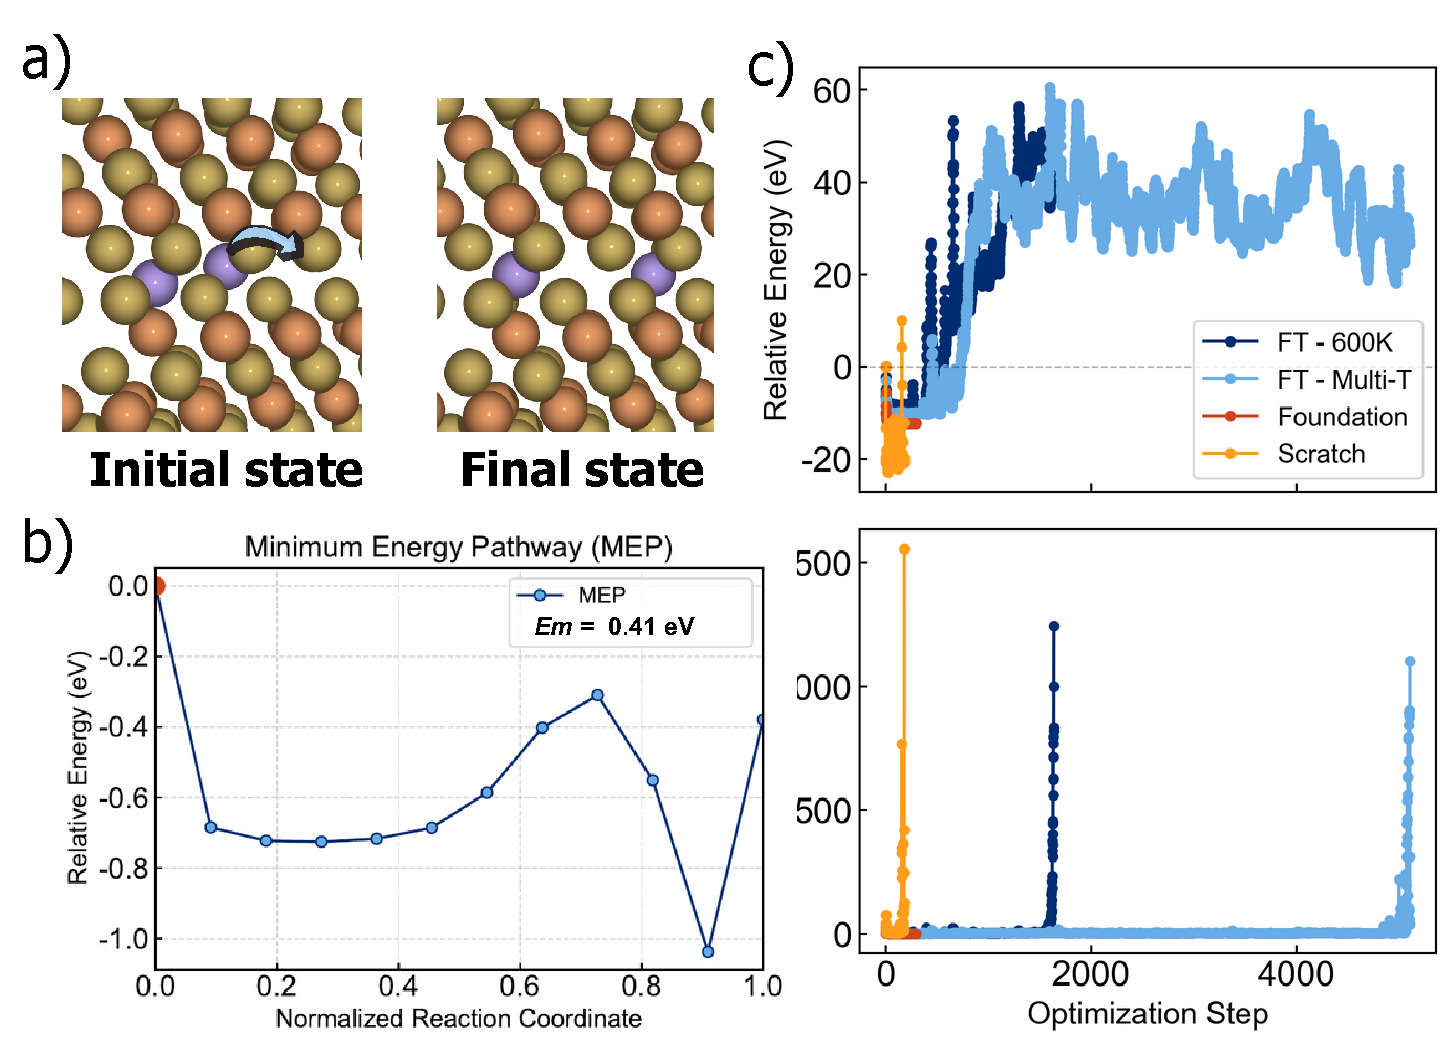
\includegraphics[width=0.8\textwidth]{Fig/NeurIPS2025-AI4MAT-SI2.pdf}
\reviewermap{REV-A1}{partial}{Caption must say model-reported MLFF barrier and distinguish self-consistent MLFF NEB from fixed-geometry DFT-path scoring.}
    \caption{Nudged Elastic Band (NEB) benchmark of MACE models for a Cr atom migration. (a) Visualization of the initial and final states of the diffusion pathway. (b) Self-consistent MEP optimized using the MACE foundation model, yielding a model-reported MLFF barrier of 0.41~eV on its own optimized band. This panel tests MLFF-NEB stability and path generation, whereas Fig.~3d in the main text tests fixed-geometry scoring on a DFT-relaxed path. (c) The evolution of the relative system energy (top panel) and the maximum force ($f_{max}$, bottom panel) during the NEB optimization for each model. The foundation model (red) converges smoothly. In contrast, the scratch (orange), FT-600K (dark blue), and FT-MultiT (light blue) models all exhibit explosive behavior, where a rapid increase in $f_{max}$ indicates instability and leads to the termination of the calculation.}
    \label{fig:neb_benchmark}
\end{figure}

\begin{figure}[htbp]
    \centering
    
\includegraphics[width=0.9\textwidth]{figures/figS_neb_pes_local_audit.pdf}
    \caption{\textbf{Local audit of self-consistent MLFF-NEB trajectory assets.} This diagnostic plot tracks the locally available scratch-model self-NEB trajectory and supports the separation between fixed-path DFT scoring and self-consistent MLFF-NEB stability. It is retained as an audit figure for Revision~1 traceability.}
    \label{fig:neb_pes_local_audit}
\end{figure}

\begin{figure}[htbp]
    \centering
    
\includegraphics[width=0.95\textwidth]{figures/figS_latent_robustness.pdf}
    \caption{\textbf{Latent-space robustness and original-descriptor checks.} The t-SNE panels show sensitivity to perplexity and seed, while the summary panel compares projected separability with original-descriptor-space silhouette scores. These checks support using the embeddings as qualitative diagnostics rather than stand-alone mechanistic proof.}
    \label{fig:latent_robustness_revised}
\end{figure}

\begin{table}[htbp]
    \centering
    \caption{\textbf{Audited SHAP surrogate fidelity.} The previous in-sample $R^2$ values are superseded by 5-fold cross-validation on the corrected 150-frame, frame-aligned surrogate workflow.}
    \label{tab:shap_surrogate_cv_revised}
    \begin{tabular}{lccc}
\toprule
Model & $n$ & 5-fold CV $R^2$ & 5-fold CV MAE (eV) \\
\midrule
FT--600K & 150 & 0.9819 & 0.03795 \\
FT--Multi-T & 150 & 0.8756 & 0.02692 \\
Scratch & 150 & 0.9730 & 0.02618 \\
\bottomrule
\end{tabular}

\end{table}

\newpage
\bibliography{sn-bibliography}

\end{document}
